% \documentclass[10pt, twocolumn]{IEEEtran}
\documentclass[11pt]{IEEEtran}
% \documentclass{llncs}

\usepackage{url}
\usepackage{graphics}

\newcommand{\workingnote}[1]{}        % The version that hides the note.
%\newcommand{\workingnote}[1]{(**#1)}   % The version that makes the note visible.

\renewcommand\url{\begingroup \def\UrlLeft{<}\def\UrlRight{>}\urlstyle{tt}\Url}
\newcommand\emailaddr{\begingroup \def\UrlLeft{<}\def\UrlRight{>}\urlstyle{tt}\Url}

% If an URL ends up with '%'s in it, that's because the line *in the .bib/.tex
% file* is too long, so break it there (it doesn't matter if the next line is
% indented with spaces). -DH

%\newif\ifpdf
%\ifx\pdfoutput\undefined
%   \pdffalse
%\else
%   \pdfoutput=1
%   \pdftrue
%\fi

\begin{document}

%% Use dvipdfm instead. --DH
%\ifpdf
%  \pdfcompresslevel=9
%  \pdfpagewidth=\the\paperwidth
%  \pdfpageheight=\the\paperheight
%\fi

\title{Mixminion: Design of a Type III Anonymous Remailer Protocol}

% Removed for anonymous review
% 
%\author{George Danezis\inst{1} \and Roger Dingledine\inst{2} \and David Hopwood\inst{3}
%        \and Nick Mathewson\inst{2}}
%\institute{Cambridge University
%\email{\emailaddr{george.danezis@cl.cam.ac.uk}}
%\and
%The Free Haven Project
%\email{\emailaddr{{arma,nickm}@freehaven.net}}
%\and
%Independent consultant
%\email{\emailaddr{david.hopwood@zetnet.co.uk}}}
\author{...}
%\institute{}

\maketitle
\pagestyle{plain} 
 
\begin{abstract}

We present Mixminion, a message-based anonymous remailer protocol that
supports secure single-use reply blocks. Mix nodes cannot distinguish
Mixminion forward messages from reply messages, so forward and reply
messages share
the same anonymity set. We add directory servers that allow users to
learn public keys and performance statistics of participating remailers,
and we describe nymservers that allow users to maintain long-term
pseudonyms using single-use reply blocks as a primitive. Our design
integrates link encryption between remailers to provide
forward anonymity. Mixminion %brings together the best solutions from
%previous work to
protects against most known attacks.

\end{abstract}

\noindent \textbf{Keywords:} anonymity, mix-net, peer-to-peer, remailer, nymserver, reply block

%%%%%%%%%%%%%%%%%%%%%%%%%%%%%%%%%%%%%%%%%%%%%%%%%%%%%%%%%%%%%%%%%%%%%%%

\section{Introduction}
\label{sec:intro}

Chaum first introduced anonymous remailers over 20 years ago
\cite{chaum-mix}. The research community has since introduced many new
designs and proofs \cite{abe}\cite{babel}\cite{flash-mix}\cite{kesdogan}\cite{shuffle}\cite{hybrid-mix},
and discovered a variety of new attacks
\cite{back-traffic-analysis}\cite{langos02}\cite{disad-free-routes}\cite{desmedt}\cite{mitkuro}\cite{raymond00}.
But because many of the newer designs require considerable coordination or
synchronization, deployed remailers still use Cottrell's Mixmaster
design from 1994 \cite{mixmaster-attacks}\cite{mixmaster-spec}. Here we describe
Mixminion, a protocol for asynchronous loosely federated remailers that
maintains Mixmaster's flexibility while addressing the following flaws:

\begin{itemize}
\item \textbf{Replies:} Mixmaster does not support replies or anonymous
recipients --- people who want these functions must use the older and
less secure Cypherpunk Type I remailer design \cite{remailer-history}. We
introduce a new primitive called a \emph{single-use reply block} (SURB),
which makes replies as secure as forward messages. Our design goes a
step further: in Mixminion most remailers in a path cannot distinguish
reply messages from forward messages. We also describe how to securely
build higher-level systems such as nymservers using these SURBs. By
integrating reply capabilities into Mixminion, we can finally retire
the Type I remailer network.

\item \textbf{Forward anonymity:} Mixmaster uses SMTP (normal mail) for
transport. We use TLS over TCP between remailers; thus we can introduce
link encryption with ephemeral keys to ensure forward anonymity for
each message. Link encryption also makes obsolete many active and
passive attacks that could have been performed on the communication
links, and forces attackers to run corrupt nodes to attack the
system. 

% We also provide flexible delivery schemes ---
%rather than just allowing delivery to mail or Usenet, we allow designers
%to add arbitrary modules to handle incoming and outgoing messages. By
%separating the core mixing architecture from these higher-level modules,
%we can both limit their influence on the anonymity properties of the
%system, and also extend the Mixminion network for uses other than
%anonymous email.

\item \textbf{Exit policies:} Exit abuse is a serious barrier to wide-scale
remailer deployment: most ISPs do not tolerate users who potentially
deliver hate mail, etc. While the original Mixmaster design assumed all
nodes have identical capabilities and roles (and thus messages can exit
from any node), Mixminion allows each node to specify an exit policy. We
describe a protocol which allows recipients to opt out of receiving mail
from remailers, but at the same time makes it difficult for an adversary
to deny service to interested recipients.

\item \textbf{Replay prevention and key rotation:} ...

\item \textbf{Integrated directory servers:} Mixmaster uses several \emph{ad hoc}
approaches to distributing remailer availability, performance, and
key information. But the fact that users and remailers operate with
different information introduces \emph{partitioning} attacks. Mixminion
uses a small group of synchronized redundant directory servers
to provide uniform information about the network.

\item \textbf{Dummy traffic:} Cottrell briefly mentions dummies in
\cite{mixmaster-attacks}, but they are not part of the specification
\cite{mixmaster-spec}. Mixminion uses a simple dummy policy which provably
improves anonymity. % compared to the absence of dummies.

\end{itemize}

%Part of the difficulty in expanding the deployed remailer base is
%due to the liability involved in running a remailer node on the Internet,
%and part is due to the complexity of the current infrastructure ---
%it is fairly hard to add new experimental features to the current software.

We review the basic mix-net protocol in Section \ref{sec:related},
and then address the above list of improvements in Sections
\ref{sec:design}-\ref{sec:nymservers}. We conclude with a list of future
work (tasks which we should do next and feel confident we can complete),
followed by a list of open questions (unresolved issues for which the
research community currently has no answer).

%The Mixminion Project aims to deploy a cleaner remailer design
%in the same spirit as Mixmaster, with the goals of expanding
%deployment, documenting our design decisions and how well they stand
%up to all known attacks, and providing a research base for
%experimental features.

%Mixminion is a best-of-breed remailer protocol that uses conservative design
%approaches to provide security against most known attacks. The overall
%Mixminion Project is a joint effort between cryptography and anonymity
%researchers and Mixmaster remailer operators. This design document
%represents the first step in peer review of the Type III remailer
%protocol.

%%%%%%%%%%%%%%%%%%%%%%%%%%%%%%%%%%%%%%%%%%%%%%%%%%%%%%%%%%%%%%%%%%%%%%%

\section{Overview and background}
%% This is a new 'overview' section to come after the toplevel
%% intro; with content as suggested by Roger.  I don't know what we
%% should rename the intro to.
%%
%% Also, the writing here NEEDS to be cleaned up.  -NM
%
% What's a MIX-net?
In a MIX-net, message senders achieve anonymity by routing their
messages through a path of relay servers, or `MIXes.'  When Alice
wants to send an anonymous message to Bob through the MIXes $M_1$,
$M_2$, and $M_3$, she encrypts her message successively with the
public keys of the mixes in reverse order, and includes routing
information for each MIX, so that each MIX $M_i$ receives the address
of $M_{i+1}$ along with the payload intended for $M_{i+1}$, all
encrypted with $M_i$'s public key.  
% This is kind of unclear.  Maybe integrate the paragraph from below
% that says 'mixminion uses the same general MIX-net paradigm...'
% 
% needs references, too

% What do MIXes do?
When a MIX receives a message, it decrypts it with its public key, 
and delays it according to some `batching rule' so that an observer
cannot easily associate its outputs with its inputs.  It then sends
extracts the address of the next MIX in the sequence from the
decrypted message, and delivers the contents of the message to the
next MIX.

% XXXX Mention how this provides any anonymity!

% What's a reply block?
When recipients want to achieve anonymity, some MIX-net designs allow
them to construct \empf{reply blocks} that allow others to send
messages to them without knowing their identities.  A reply block
contains only the routing portion of a message; the actual contents
are provided by the user that eventually sends a message to the
recipient.

% How does mixminion fit in?
Mixminion's principal difference from earlier MIX-net designs is the
mechanism it uses to support reply messages with the same processing
machinery as non-reply messages, while at the same time resisting the
attacks described below in REF.
% This could be phrasesd far better

\subsection{Design goals and assumptions}
% this needs more material, and a bit less 'attitude' :)

% Server requirements
First of all, the system must be relatively simple to deploy.  Past
systems have never found it easy to get a reliable pool of MIX
operators to run long-lived servers; Mixminion must add as few
technical barriers as possible.  Thus, we require that our protocol
require only loose clock synchronization (within a few minutes);
that it achieve acceptable performance on commodity hardware, and 
that it require little coordination between servers.

% Client requriements
Furthermore, software adoption has also been a barrier to past
systems. (REF?) Thus, we require that only users who receive anonymity
from the system need to run special software -- that is, users should
be able to receive messages from anonymous senders and send messages
to anonymous recipients without any support beyond a standard email
client.  Users must also be able to send and receive anonymous
messages using only commodity hardware.  Finally, although users with
persistant network connections are necessarily more resistant to
intersection attacks than users with intermittent connections (see
REF below), the system must still support users with intermittent
connections and offer them as much anonymity as possible.

For an adversary model, we assume a well-funded attacker who can
observe all or most traffic on the network, who can generate, modify,
delete, or delay traffic on the network, who can operate MIXes of its
own, and who can compromise some fraction of the MIXes on the network.
We assume that such an adversary is attempting to compromise users'
anonymity by learning (or guessing with a reasonable probability) who
is communicating with whom.
%What else is the adversary trying to do?

We want to resist

replies: we want to avoid partitioning by having reply messages be
   indistinguishable from forward messages, and just as secure.  To the
   extent possible, a MIX should not be able to learn any more from a
   message's contents than from the fact of the message's receipt.


\subsection{Known attacks against MIX-nets}

The largest class of passive attacks against 

-control servers
-compromise servers

-replay

-delaying
-dropping
-textual analysis

-partitioning

-tagging attacks

-(n-1) attack

-directory-related attacks

-flooding attack

-delaying attack

-timing attacks

-intersection attacks

%%%%%%%%%%%%%%%%%%%%%%%%%%%%%%%%%%%%%%%%%%%%%%%%%%%%%%%%%%%%%%%%%%%%%%%

\section{Related Work}
\label{sec:related}

\subsection{MIX-nets}

Chaum introduced the concept of a MIX-net for anonymous communications
\cite{chaum-mix}. A MIX-net consists of a group of servers, called
MIXes (or MIX nodes), each of which is associated with a public
key. Each MIX receives encrypted messages, which are then decrypted,
batched, reordered, and forwarded on without any information
identifying the sender. Chaum demonstrates the security of MIXes
against a \emph{passive adversary} who can eavesdrop on all
communications between MIXes but is unable to observe the reordering
inside each MIX.

Recent research on MIX-nets includes stop-and-go MIX-nets
\cite{kesdogan}, distributed flash MIXes \cite{flash-mix} and their
weaknesses \cite{desmedt}\cite{mitkuro}, and hybrid MIXes \cite{hybrid-mix}.

One type of MIX hierarchy is a cascade.
In a cascade network, users choose from a set of fixed paths through
the MIX-net.
Cascades can provide greater anonymity against a large adversary:
free-route systems allow an adversary who owns many MIXes to use
intersection attacks to reduce the set of possible senders or receivers
for a given
% still not quite worded well. -RRD
message \cite{disad-free-routes}. On the other hand, cascades are more
vulnerable \cite{batching-taxonomy} to trickle attacks, where an attacker
targeting a specific message going into a MIX can manipulate the batch
of messages entering that MIX so the only unknown message in the batch
is the target message \cite{mixmaster-attacks}\cite{babel}.
MIX cascade research includes real-time MIXes \cite{realtime-mix} and
web MIXes \cite{web-mix}. Even when not under attack cascades will
provide smaller anonymity sets than networks since the least
resourceful acts as a traffic bottleneck.

\subsection{Deployed Remailer Systems}

The first widespread public implementations of MIXes were produced by the
Cypherpunks mailing list. These ``Type I'' \emph{anonymous remailers}
were inspired both by the problems surrounding the {\tt anon.penet.fi}
service \cite{helsingius}, and by theoretical work on MIXes. Hughes wrote
the first Cypherpunk anonymous remailer \cite{remailer-history}; Finney
followed closely with a collection of scripts that used Phil Zimmermann's
PGP to encrypt and decrypt remailed messages. Later, Cottrell implemented
the Mixmaster system \cite{mixmaster}\cite{mixmaster-spec}, or ``Type II'' remailers,
which added message padding, message pools, and other MIX features lacking
in the Cypherpunk remailers. Note that Mixmaster does not include replies,
so deployed remailer systems still use the less secure
long-term Cypherpunk reply blocks.

At about the same time, Gulcu and Tsudik introduced the Babel
system \cite{babel}, a practical remailer design with many desirable
features. While it provides replies, they are only indistinguishable
from forward messages by passive observers; the MIX nodes can still
distinguish. Babel's reply addresses are multiple-use, making them less
secure than forward messages due to replay vulnerabilities. Babel also
introduces \emph{inter-MIX detours}, where nodes can rewrap a message
and send it through a few randomly chosen new hops --- so even the sender
cannot be sure of recognizing his message as it leaves the MIX.

%\subsection{Robustness}
%
%Previous work primarily investigates the \emph{robustness} of MIX-nets
%in the context of a distributed MIX system \cite{flash-mix}. A MIX
%is considered robust if it survives the failure of any $k$ of $n$
%participating servers, for some threshold $k$. This robustness is
%all-or-nothing: either $k$ servers are good and the MIX works, or they are
%not good and the MIX likely will not work.
%
%Robustness has been achieved primarily via zero-knowledge proofs of
%correct computation.  Jakobsson showed how to use precomputation to reduce
%the overhead of such a MIX network to about 160 modular multiplications
%per message per server \cite{flash-mix}, but the protocol was later
%found to be flawed \cite{mitkuro} by Mitomo and Kurosawa.  Desmedt and
%Kurosawa's alternate approach \cite{desmedt} requires many participating
%servers. Abe's MIX \cite{abe} provides \emph{universal verifiability} in
%which any observer can determine after the fact whether a MIX cheated,
%but the protocol is still computationally expensive. Neff recently
%made further efficiency improvements to universally verifiable mixing
%\cite{shuffle}.

\subsection{Remailer Statistics}

Levien's \emph{statistics pages} \cite{levien} track both remailer
capabilities (such as what kinds of encryption the remailer supports)
and remailer up-times (obtained by pinging the machines in question
and by sending test messages through each machine or group of
machines).  Such \emph{reputation systems} improve the reliability of
MIX-nets by allowing users to avoid choosing unreliable MIXes. The
Jack B Nymble 2 remailer client \cite{potato} and the Mixmaster 2.9
remailer allow users to import statistics files and can then pick
remailers according to that data. Users can specify minimum
reliability scores, decide that a remailer should always or never be
used, and specify maximum latency. Ongoing research on more powerful
reputation systems includes a reputation system for free-route
networks \cite{mix-acc} and another for MIX cascades \cite{casc-rep}.

%%%%%%%%%%%%%%%%%%%%%%%%%%%%%%%%%%%%%%%%%%%%%%%%%%%%%%%%%%%%%%%%%%%%%%%

\section{The MIX-net Design}
\label{sec:design}

Mixminion brings together the current best approaches for providing
anonymity in a batching message-based MIX environment. We don't aim
to provide low-latency connection-oriented services like Freedom
\cite{freedom} or Onion Routing \cite{goldschlag99} --- while those
designs are more effective for common activities like anonymous web
browsing, the low latency necessarily implies smaller anonymity sets
than for slower message-based services. Indeed, we intentionally
restrict the set of options for users: we provide only one
cipher suite, and we avoid extensions that would help an adversary
divide the anonymity set.

Mixminion uses the same general MIX-net paradigm as previous work
\cite{chaum-mix}\cite{mixmaster-attacks}\cite{babel}. The sender Alice chooses a
path through the network. She repeatedly ``onion'' encrypts her message,
starting with the last
MIX in her path, and sends the onion to the first MIX. Each
MIX unwraps a single layer of the onion, pads the message to a fixed
length (32 Kbytes in our current design), and passes the result to the
next MIX. We describe the behavior of the last MIX in
Section \ref{subsec:delivery-modules}.

% A bit more detail about what is contained in the header: -George

Headers addressed to each intermediate MIX are encrypted using RSA.
%RSA-OAEP \cite{PKCS1} and are of 128 bytes each.
% IMO we should use OAEP+, and variable-length headers. -DH
They contain a secret 
that can be used to generate padding and decrypt the rest
of the message. They also contain the address of the next node to 
which the message should be forwarded along with its expected signature 
key fingerprint.

% we haven't said what a subheader is yet. too early to say this. -RD
%To frustrate tagging attacks (see
%Section \ref{subsec:tagging}), the sub-header also contains a hash of
%the header.

% This last paragraph assumes that the audience already knows the
% material well enough to know that Alice encrypts each layer with the
% appropriate MIX's public key. Is this assumption safe -Nick

While Mixminion protects against known \emph{traffic analysis} attacks
(where an adversary attempts to learn a given message's sender or
receiver \cite{rackoff93cryptographic}\cite{raymond00}), we do not fully
address \emph{traffic confirmation} attacks. In a traffic confirmation
attack, the adversary treats the MIX network as a black box and
observes the behavior of senders and receivers. Over time, he can
intersect the set of senders and receivers who are active at certain
times and learn who is sending and receiving which messages
% Really?  I thought that an intersection attack told you who was
% talking with whom, not which messages were sent to whom.  I.e., Eve
% can learn that Alice is sending messages to Bob and Carol, but
% can't be certain which messages were meant for whom. -Nick
% But if we further intersect to learn that the messages on Tuesday
% are for Bob and those on Wednesday are for Carol, ... -RRD
\cite{langos02}. Good dummy traffic designs may eventually address the
intersection attack, but for now it remains an open problem.

We choose to drop packet-level compatibility with Mixmaster and the
Cypherpunk remailer systems, in order to provide a simple extensible
design. We can retain minimal backwards compatibility by ``remixing''
Type II messages to be Type III messages, thus increasing anonymity
sets in the Type III network. Type II messages travelling between
Type III remailers are treated
as plaintext and encrypted to the next remailer in the chain using its
Type III key. The message is sent as a Type III encrypted message, but
it decrypts to reveal the Type II message.

We also provide a new feature: a reply block mechanism that is as secure
as forward messages.
Reusable reply blocks, such as those in the Cypherpunk remailer, are a
security risk --- by their very nature they let people send multiple
messages through them.  These multiple messages can easily be used to
trace the recipient's path: if two incoming batches both include a
message to the same reply block, then the next hop must be in the
intersection of both outgoing batches.  To prevent these replays,
Mixminion therefore provides only \emph{single-use} reply blocks. Since
replies may be very rare relative to forward messages, and thus
much easier to trace, the Mixminion protocol makes reply messages
indistinguishable from forward messages even for the MIX nodes. Thus
forward and reply messages can share the same anonymity
set. Unfortunately reply blocks are fundamentally more dangerous than
forward secure communications due to the fact that the adversaries have
in their possession a string that they can force intermediate mixes to
decrypt until the originator is reached.

\subsection{Tagging attacks}
\label{subsec:tagging-attacks}

To motivate some aspects of the Mixminion design, we describe an attack
that works against many MIX-net protocols, including Mixmaster and Babel.

A {\em tagging attack} is an active attack in which a message is
modified by altering part of it (for example by flipping bits), so
that it can be recognized later in the path.  A later MIX controlled by
the attacker can recognize tagged messages because the header does
not conform to the expected format when decrypted.  Also, the final
recipient can recognize a tagged message for which the payload has
been altered.

Checking the integrity of hop headers individually is not
sufficient to prevent tagging attacks.  For example, in Mixmaster
each hop header contains a hash of the other fields in that header
\cite{mixmaster-spec}.
Each MIX in the path checks the integrity of the header, and drops
the message immediately if it has been altered.  However, 
an attacking MIX can still alter a header that will be decrypted
only after several more hops, and so tagging attacks are still possible.

The most straightforward way to prevent tagging attacks is to
verify the integrity of the whole message at every hop.  For forward messages,
then, the padding added to a message must be derived deterministically,
so that it is possible to calculate
authentication tags for the whole message at each hop.  But
the situation becomes more complicated when reply messages are
introduced --- the message and the reply block are
created by different users. It is therefore impossible for the creator
of the SURB to include in the header a checksum of a message it they
do not yeat know. Mixminion uses a hybrid strategy to protect against
such attacks, by protecting the headers using cryptographic checksums,
while making sure that the addressing information contained in the
message is destroyed if the payload is modified by an adversay.

\subsection{Replies}
\label{subsec:replies}

The rest of this section describes the mechanism for secure replies,
including how we defeat tagging-related attacks. Mixminion's reply
model is in part inspired by Babel \cite{babel}, as it requires the
receiver of a reply block to keep no other state than its secret keys,
in order to read the reply.  All the secrets used
to strip the layers of encryption are derived from a master
secret contained in the last header of the single-use reply block, which
the creator of the block addresses to itself and encrypts under its
own public key.

\subsection{Indistinguishable replies}
\label{subsec:header-swap}

By making forward messages and replies indistinguishable even to MIXes,
we prevent an
adversary from dividing the message anonymity sets into two classes. In
particular, if replies are infrequent relative to forward messages,
an adversary who controls some of the MIXes can more easily trace the
path of each reply.

Having indistinguishable replies, however, makes it more difficult to
prevent tagging attacks.  Since the author of a reply block is not the
one writing the payload, a hash of the entire message cannot be used.
Therefore, since we choose to make forward messages and replies
indistinguishable, we cannot include hashes for forward messages either.
Our approach to defending against these attacks is discussed in more
detail in Section \ref{subsec:tagging-defenses}.

Mixminion allows Alice to send messages to Bob in one of three ways:

\begin{enumerate}
\item \textbf{Forward} messages where only Alice remains anonymous
($(A) \rightarrow B: M$.) 
\item \textbf{Direct Reply} messages where only Bob remains anonymous 
($A \rightarrow (B): M$.)
\item \textbf{Anonymized Reply} messages where Alice \emph{and} Bob
   remain anonymous ($(A) \rightarrow (B): M$.)
\end{enumerate}

We require parties that benefit from anonymity properties to run dedicated
software.  Specifically, senders generating forward messages must be able
to create onions, and anonymous receivers must be able to create reply blocks
and unwrap messages received through those reply blocks. Other parties,
such as those receiving forward messages and those sending direct reply
messages, do not need to run new software. (The quoting
performed by ordinary mail software can be used to include the reply
block in a direct reply; this is sent to a node at the Reply-To:
address, which extracts the reply block and constructs a properly
formatted onion.)

\begin{figure}
\begin{center}
\resizebox{15cm}{!}{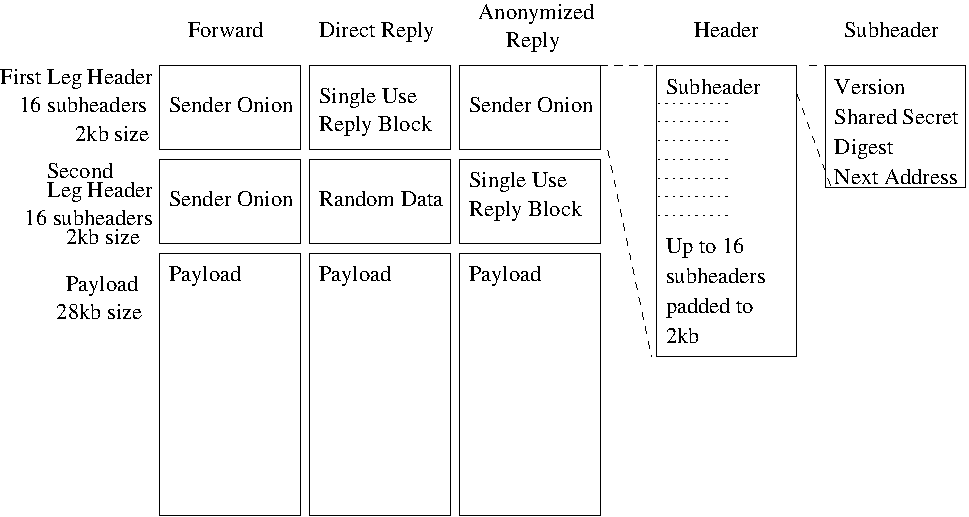
\includegraphics{headerDiagram}}
\caption{The header configurations for different anonymity functions.} 
\end{center}
\end{figure}

Messages are composed of a header section and a payload. We divide
a message's path into two \emph{legs}, and split the header section
correspondingly into a main header and a secondary header. Each header
is composed of up to 16 subheaders, one for each hop along the path.
Each subheader contains a hash of the remainder of its header as
seen by the appropriate MIX, so we can do
integrity-checking of the path (but not the payload) within each leg.
Each subheader also contains a symmetric key, which is used to derive a
decryption key for decrypting the rest of the message. The MIX also
derives a padding seed from this master key. It uses this padding seed
to place predictable padding at the end of the header, so the hash will
match even though each hop must regrow the header to maintain constant
length.

For forward messages, Alice provides both legs; for anonymous replies, Alice
uses Bob's reply block as the second leg, and generates her own path
for the first leg.  To send a direct reply, Alice can use an empty
first leg, or send the reply block and message to a MIX that can wrap
them for her.

When Alice creates her message, she encrypts the secondary header
with a hash of her payload (in addition to the usual layered onion
encryptions). Alice's message then traverses the MIX-net as normal (every
hop pulls off a layer, verifies the hash of the current header,
and puts some junk at the end of the header), until it gets to a
hop that is marked as a \emph{crossover point}. This crossover point
performs a ``swap'' operation: it decrypts the secondary header with
the hash of the current payload, and then swaps the two headers. The
swap operation is detailed in Figure 1 --- specifically, the normal
operations done at every hop are those above the dotted line, and the
operations performed only by the crossover point are those below
the dotted line. The encryption primitive, labelled ``LBC'', that is
used to blind the second header and the payload needs to have certain
properties:

\begin{itemize}
\item it is length-preserving;
%\item it behaves like an all-or-nothing transform on the whole of
%      the message;\footnote{Except that we need a keyed primitive,
%      whereas an all-or-nothing transform is normally unkeyed, and
%      not length-preserving.}
%% I think that if we have the next item, we don't need this. -DH

\item it should be impossible to recognize the decryption of a modified
      block, without knowledge of the key;
%what the heck does this mean? i don't know what 'the key' is. this is
%probably too imprecise for us.
\item it should be equally secure to use the decryption operation
      for encryption.
\end{itemize}

To fulfill the above requirements we use a variable length block
cipher adapted to the length of the payload; that
is, a cipher that acts as a permutation on a block the size of its
input (a header or the payload).  Possible candidates
include LIONESS \cite{BEAR-LIONESS} and SPC \cite{SPC}.
The cryptographic property required is that of a super-pseudo-random
permutation (a.k.a. strong pseudo-random permutation) or SPRP \cite{sprp}.\footnote{
The weaker PRP property may be sufficient, given that preventing
replays limits the number of oracle queries to 1; this will need
further analysis.  In that case the simpler BEAR construction
\cite{BEAR-LIONESS} could be used instead of LIONESS.}
Thus if any bit of
the encrypted material is changed, the decryption will look like random
bits.  An SPRP is also equally secure in the encryption and decryption
directions.  See Section \ref{subsec:tagging-defenses} for a
discussion of how this approach helps protect against tagging.

% BEAR isn't an SPRP; LIONESS is. I'm not sure that an SPRP is necessary,
% but I'm sure that it is sufficient. We don't need encryption and
% decryption to be the same. -DH

%To fulfill the above requirements we use a variable block size block cipher
%named BEAR [2] as our encryption and decryption primitive. BEAR offers the
%property that if any bit of the encrypted material is changed, the decryption
%will look like random bits. We can use BEAR in a mode where decryption and
%encryption are equivalent, by using the same key for both of its hash steps.
%
% ``Both hash steps''?  We never mention Bear's hash steps... -Nick
% True. Does adding 'its' help? -RRD
% Adding 'of' helps more for me.  Also, doesn't George once have a
% source for this? -Nick


\begin{figure}
\begin{center}
\resizebox{10cm}{!}{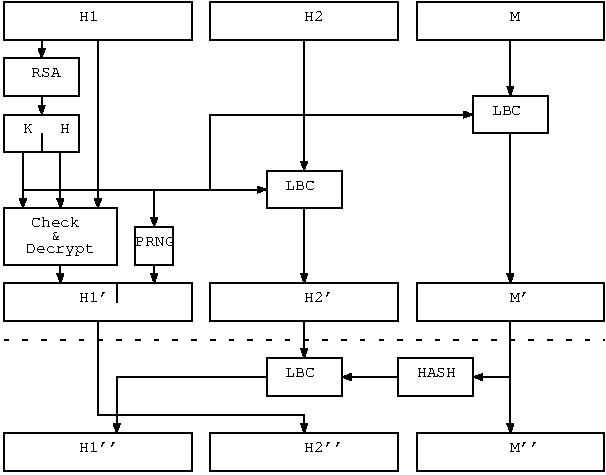
\includegraphics{SWAP}}
\caption{The operations required by the ``swap'' method} 
\end{center}
\end{figure}


\subsection{Defenses against tagging attacks}
\label{subsec:tagging-defenses}

Without the crossover point, an adversary could mount a tagging
attack by modifying the payload of a forward message as
it leaves Alice, and recognizing it later when it reaches Bob.
Specifically, if our encryption mechanism were an ordinary
counter-mode cipher, he might alter a specific byte in the payload of
a message entering the MIX-net. Since many of the outgoing messages
will be in part predictable (either entirely plaintext, or with
predictable PGP header material), the adversary can later observe
messages exiting the MIX-net and look for payloads that have a
corresponding anomaly at that byte.

% I think we shold point out =someplace= why we can't use
% CBC or anything else that isn't symmetrically good for encryption
% and decryption.  -Nick

We use a large-block cipher as described in the previous section to
minimize the amount of information an adversary can learn from tagging.
If he tags a message
leaving Alice, the payload will be entirely random when it reaches
Bob.  Thus, an adversary who tags a message can at worst turn the
corresponding payload into trash.  
%%Thus if he tags more than one message in the entire MIX-net, he
%%learns only one bit from each tagged message, so he cannot distinguish
%%the tagged messages. 
% I think that the above sentence raises more objections than it 
% addresses; thus, I'm omitting it.  The real security comes from the
% crossover step as described below.  Without the crossover
% decryption, BEAR is insufficient, and one bit is too much. -Nick
%Nevertheless, this may still allow an adversary to
%break anonymity in some cases.

We briefly considered introducing \emph{cover-trash}, dummy messages
designed to look like tagged messages, to frustrate
these tagging attacks; but that problem is as complex as the dummy
traffic problem \cite{langos02}. Instead, we use the
% decryption-by-hash-of-payload 
``swap'' step at the
crossover point to prevent the attacker from learning information from
tagging attacks. The second header of the message, that contains the
path to the final destination of the forward path,  is encrypted by the
sender by the hash of the payload that is to arrive at the mix. The
mix then needs to perform the decryption and swap the first header for
the second one.
Specifically, our solution falls into several cases:

\begin{itemize}
\item Forward messages: if the message is tagged during the first leg,
the second header is unrecoverable, and so the adversary cannot
learn the intended destination of the message. If the message is tagged
during the second leg, then the first leg has already provided anonymity,
and so the adversary cannot learn the sender.
\item Direct reply messages: since the decryption algorithm provides
secrecy equivalent to encryption, the effect is similar to {\em encrypting}
the payload at each step along a reply block. Only the recipient can learn,
after peeling off all layers, whether the message has been tagged. Thus
tagging attacks are useless against reply messages.
\item Anonymized reply messages: as with forward messages, if the first leg
is tagged the second header is unrecoverable --- so an adversary will
never learn that the message was addressed to a reply block. And as with
direct reply messages, only the recipient can learn if the second leg is
tagged.
\end{itemize}

While direct reply messages do not need a crossover point in the path
(the adversary can never observe his tag), forward messages still need a
crossover point to prevent end-to-end tagging. But since the first leg
either provides sufficient anonymity or destroys the information about
the second leg, the second leg in a forward message can be very short.
At the extreme, the first hop in the second header could directly
specify the message recipient. However, the choice of crossover point
can still reveal information about the intended recipient,\footnote{For instance,
some MIXes may only allow outgoing mail to local addresses; if such a
node gets a crossover message that has been trashed, it might guess
that the recipient is one of the local addresses.} and so we recommend
that the second leg be at least a few hops long.

No MIX except the crossover point can distinguish forward messages from
replies --- even the crossover point cannot be sure whether it is processing
a reply or forward message, but it may be able to guess that crossover
points are more frequent on forward paths than direct replies or
anonymized reply paths.
%The protocol doesn't allow a MIX to know its location in the path (other
%than the exit node), or the total length of the route.
% [WE NEED TO SAY THIS SOMEWHERE SINCE IT IS AN IMPORTANT FEATURE! -GD]

\subsection{Multiple-message tagging attacks}
\label{subsec:multi-tagging}

The above design is still vulnerable to a subtle and dangerous
attack. If Alice sends a group of messages along the same path, the
adversary can tag some of those message as they leave Alice, recognize
the pattern (number and timing of tagged and untagged messages) at the
crossover point, and observe where the untagged ones go.
% (if he built
%the second leg himself, as in an anonymized reply, he can recognize
%it immediately).
With some assumptions about our adversary, we can reduce
this attack to a traffic confirmation attack we're already willing to
accept: when Alice sends a bunch of messages, the adversary can count
them and look for the pattern later. He can also drop some of them and
look for resulting patterns.

The adversary can only recognize a tag if he happens to own the crossover
point that Alice chooses.
Therefore, Alice picks $k$ crossover points for her
messages;\footnote{
  We can prevent the adversary from using divide-and-conquer on Alice's
  groupings if Alice uses a hybrid path starting with a short cascade ---
  so even if the adversary tags a subset of the messages he doesn't know
  (unless he owns the whole cascade) the groupings of tagged messages.
}
to match a tag signature with certainty an adversary would
have to own all $k$ crossover points.  (And even then, it seems harder
as the subsets of her messages would overlap with subsets of
messages from other senders.)

% The argument above seems a little handwavy to me.  We should either
% expand it to say why the adversary needs certainty to mount the
% multiple-messages attack, or express less confidence in it.  I'm
% taking the latter route below, and changing ``is infeasible''
% to ``seems infeasible''  -Nick

The key here is that when the adversary doesn't own a given crossover
point, tagging messages destined for that crossover is equivalent to
dropping them.  The crossover point in question simply doesn't deliver
the message to the second leg. Therefore, if the adversary doesn't own
most of the crossover points that Alice chooses, a successful
multiple-message tagging attack seems infeasible.  We leave a security
analysis of the multiple-paths idea to future work; but see
Section \ref{sec:maintaining-anonymity}.

\section{Related design decisions}

%In this section we discuss how we are using
%link encryption with ephemeral keys to provide forward anonymity,
%message types and modules to handle different types of messages, and
%exit policies for advertising what delivery options a node will provide.

\subsection{Link encryption and what it gets us}
\label{subsec:link-encrypt}

Unlike remailer Types I and II that used SMTP \cite{SMTP} (i.e. ordinary
Internet e-mail) as their underlying transport mechanism, Mixminion
clients and nodes communicate using a forward secure encrypted channel
based on TLS \cite{TLS}.  
TLS allows the establishment of an encrypted tunnel using ephemeral
Diffie-Hellman keys. In order to guarantee that the receiving end is
the one intended by the creator of the anonymous message, the
receiving node signs the ephemeral key. As soon as a session key
has been established, the parties destroy their Diffie-Hellman keys
and begin sending messages through the tunnel. After each message, the
parties perform a standard key update operation to generate a fresh
key, and delete the old key material.  Key updates don't require any
asymmetric encryption techniques, so they are relatively fast.

% Do we want to specify how much of the above happens with TLS
% Handshake/ChangeCipherSpec packets, and how much happens within the 
% application data?  I =believe=[*] that TLS can do all of the above with 
% standard stuff; do we want to use TLS vocabulary to convince
% people? 
%
%  [*]My only reservation is doing key updates without assymetric
%  encryption.  I need to doublecheck that such an operation is really 
%  specified in the RFC.                               -Nick
%  It is: the server can send a HelloRequest or the client a
%  ClientHello at any time. -DH.


% Also, do we want to specify a required level of encryption?  It
% would be pretty useless if we allowed export or null ciphers
% suites.
%
% One of these modes (specified in ietf-tls-ciphersuite-03.txt) is
% probably best for us:
%             (A)   ``DHE-DSS-AES128-SHA''
%             (A)   ``DHE-RSA-AES128-SHA''
%             (B)   ``ADH-AES-128-SHA''
%             (A)   ``DHE-DSS-AES256-SHA''
%             (A)   ``DHE-RSA-AES256-SHA''
%             (B)   ``ADH-AES256-SHA''
% I'm not sure, though, whether we want one of the cert-based ones (A)
% or one of the the anon-server ones. (B) -Nick

The purpose of link encryption is to provide forward secrecy: 
after the keys have been deleted, not even the
nodes that exchange messages can decrypt or recognize messages
that might have been intercepted on the links. This makes it
impossible to comply with decryption notices of past traffic 
that might be served in
some jurisdictions.  
%It also forces adversaries to 
%corrupt and control nodes in order trace
%a forward anonymous communication by requesting nodes to decrypt
%it. 
%   I removed these sentences. If somebody knows what we meant,
%   feel free to fix that. :) -RRD
% In advance, or later?  I'm not clear what the above sentence is
% saying. -Nick
%(Reply blocks can still be used for this purpose.)
Even if an
attacker manages to get hold of the session key at a particular point
they would have to observe all subsequent traffic to be able to update
their key appropriately.

Additionally link encryption makes active and passive attacks on the
network links very difficult. Given that mix messages give an
indication to the mixes about the identity of their successors it is
hard for an 
adversary to modify messages, inject messages in a node as if they
were part of the normal communications, or delete messages. It is
still possible to delay messages, unless an additional
\emph{heartbeat} signal is included in the SSL tunnel. This forces a
determined adversary to run nodes or to corrupt nodes in 
order to break the anonymity of mixminion.

The encrypted channel offers only limited protection against traffic
analysis. Encrypted links between honest nodes prevent an adversary
from recognizing even his own messages; but without link padding, he
can still measure how much traffic is being transmitted.

As a fringe benefit, using a separate link protocol makes it
easier to deploy relay-only MIXes --- such nodes simply omit SMTP
support.  (See Section \ref{subsec:delivery-modules} below.)
% Credit for the above point goes to Len.

\subsection{Message types and delivery modules}
\label{subsec:delivery-modules}

[I think it is important to say what modules get us in comparison to
normal client side mixminion (which servers can also use). In
particular, access to some shared key material and plug-in for
infrastructure critical services. -GD]

Once a Mixminion packet reaches the final MIX in its path, it must
either be delivered to its intended recipient, dropped if it is an
intra-network dummy message, or processed further if it is a remixed
Type II packet. In order to support different kinds of
delivery, the header includes a type code for the action to be taken
to deliver the message.  A few types --- such as `dummy', `SMTP', and
`local delivery' --- are specified as a part of the Mixminion
standard.  Others may be added by future extensions, to
implement abuse-resistant exit policies (see Section
\ref{subsec:exitpolicies}), to administer nymservers (see Section
\ref{sec:nymservers}), to publish anonymously to Usenet, to relay
messages to older remailers, or to support other protocols.

Nearly all delivery methods require additional information beyond the
message type and its payload.  The SMTP module, for example, requires
a mailbox.\footnote{A {\it mailbox} is the canonical form of the
``{\tt user@domain}'' part of an e-mail address. Mixminion uses only
mailboxes in the protocol, because the display name and comment parts
of an e-mail address could potentially be different for senders who
have obtained an address from different sources, leading to smaller
anonymity sets.}
This information is placed
in a variable-length annex to the final subheader.

%\footnote{It must be
%in the header, since putting delivery information in the payload would
%prevent people from creating SURBs that can be delivered by SMTP.
%On the one hand, under the ``header swap'' method described in
%\ref{subsec:header-swap}, the all-or-nothing property of BEAR prevents
%the generator of a reply block from putting any information in the
%payload.  On the other hand, under the ``distinguish replies'' method
%in \ref{subsec:distinguish-replies}, the delivery information would
%create a portion of the payload that the final node could
%distinguish from random garbage, thus allowing a tagging attack
%against the reply block.}.
%
% See my messages of April 9 and 10 titled ``SMTP service'' for a more
% detailed version of the above argument. -Nick
%
% Should we say _why_ it's undesirable to force reply recipients to
% run local nodes?  [My answer is (A) that some people (such as human
% rights activists using internet cafes) want to get replies, but
% don't have persistent net connections, (B) that Mixmaster
% supports it, and not doing so would be a step backwards, and (C)    
% that there's not much reason not to.]    -Nick
%%%%%%
% The above footnote and comments comment, deleted by RRD, re-added by
% DH, is of historical interest only. :)  Nonetheless, it's still a
% subtle point.  Mixmaster  puts the delivery info in the payload; 
% someplace, perhaps in a different  document, we should explain why 
% we don't.  -Nick

The types each MIX supports are described in a \emph{capability block},
which also includes the MIX's address, long-term (signing) public key,
short-term public key (for use in header encryption), remixing capability,
and batching strategy. MIXes sign these capability blocks
and publish them on directory servers (see Section \ref{sec:dir-servers}).
Clients download this information from the directory servers.

% Is all of the stuff above really in the caps block?  Or do we break
% the volatile part (short-term key) from the nonvolatile part? -Nick
%
% I think they should be in the same block, although probably
% "capability block" isn't a good name for it. Capabilities should
% also be able to change without losing identity/reputation, and
% there would be no point in having two separate update mechanisms. --DH

The possibility of multiple delivery methods doesn't come free: their
presence may fragment the anonymity set.  For example, if there were five
ways to send an SMTP message to Bob, an attacker could partition Bob's
incoming mail by guessing that one of those ways is Alice's favorite.
An active attacker could even lure users into using a compromised
exit node by advertising that node as supporting a
rare but desirable delivery method.

We claim that these attacks do not provide an argument against
extensibility \emph{per se}, but rather argue against the proliferation
of redundant extensions, and against the use of rare extensions.  

\subsection{Exit policies and abuse}
\label{subsec:exitpolicies}

One important entry in a node's capability block is its \emph{exit
policy}. Exit abuse is a serious barrier to wide-scale remailer deployment
--- rare indeed is the network administrator tolerant of machines that
potentially deliver hate mail. % to the U.S. President.

On one end of the spectrum are \emph{open exit} nodes that will
deliver anywhere; on the other end are \emph{middleman} nodes that
only relay traffic to other remailer nodes and \emph{private exit}
nodes that only deliver locally. More generally, nodes can set
individual exit policies to declare which traffic they will let exit
from them, such as traffic for local users or other authenticated
traffic \cite{onion-discex00}.

Preventing abuse of open exit nodes is an unsolved problem. If
receiving mail is opt-in, an abuser can forge an opt-in request from
his victim. Indeed, requiring recipients to declare their interest
in receiving anonymous mail is risky --- human rights activists in
Guatemala cannot both sign up to receive anonymous mail and also retain
plausible deniability.\footnote{
  Compare with the 1965 U.S. Supreme Court case Lamont v. Postmaster
  General (381 U.S. 301), where the Post Office would detain mail it
  deemed to be `communist political propaganda' and instead send a form
  to the addressee telling him to send back the signed form if he wanted
  to receive such mail. The government maintained a list of citizens
  who had filled out these forms.
} Similarly, if receiving mail is opt-out, an abuser can deny service
by forging an opt-out request from a legitimate user. We might instead
keep the mail at the exit node and send a note to the recipient
telling them how to collect their mail; but this increases
server liability by storing messages (see Section \ref{sec:nymservers}
below), and also doesn't really solve the problem.

Of course, a mixture of open and restricted exit nodes will allow the
most flexibility for volunteers running servers. But while a large number
of middleman nodes is useful to provide a large and robust network, the
small number of exit nodes still simplifies traffic confirmation
(the adversary observes both a suspected user and the
network's exit nodes and looks for timing or packet correlations). The
number of available open exit nodes remains a limiting security parameter
for the remailer network.

\subsection{Replay prevention, message expiration, and key rotation}

Mixmaster offers rudimentary replay prevention by keeping a list of recent
message IDs. To keep the list from getting too large, it expires entries
after a server-configurable amount of time. But if an adversary records
the input and output batches of a MIX and then replays a message after
the MIX has forgotten about it, the message's decryption will be exactly
the same. Thus, Mixmaster does not provide the forward anonymity that we want.

Chaum first observed this attack in \cite{chaum-mix},
but his solution (which is proposed again in Babel\footnote{
  Actually, Babel is vulnerable to a much more direct timestamp attack:
  each layer of the onion includes ``the number of seconds
  elapsed since January 1, 1970 GMT, to the moment of message composition
  by the sender.'' Few people will be composing a message on a given
  second, so an adversary owning a MIX at the beginning of the path and
  another at the end could trivially recognize a message.
}) --- to include in each message a timestamp that describes when that message
is valid --- also has problems. Specifically, it introduces a new class
of \emph{partitioning} attacks, where the adversary can distinguish and
track messages based on timestamps. If messages have short lifetimes,
legitimate messages may arrive after their expiration date and be
dropped. But if we specify expiration dates well after when we expect
messages to arrive, messages arriving near their expiration date will be
rare: an adversary can delay a message until near its expiration date,
then release it and trace it through the network.

% need to read stop & go mix paper here. -RRD

One way of addressing this partitioning attack is to add dummy traffic
so that it is less rare for messages to arrive near their expiration date;
but dummy traffic is still not well-understood. Another approach would
be to add random values to the expiration date of each MIX in the path,
so an adversary delaying a message at one MIX cannot expect that it
is now near to expiring elsewhere in the path; but this seems open to
statistical attacks.

% Partitioning can be prevented completely using synchronous batching.
% Client software just needs to know the current time accurate to one
% batch period (e.g. one UTC day), and even if it gets that wrong, the
% message will just be dropped by the first honest node on the route.
% --DH
% True. We need to think more on the tradeoffs of the synchronous batching
% approach. It's definitely a good thing to mention. I've uncommented the
% below for now so readers can have a complete paper. -RRD

A possible compromise solution that still provides forward anonymity
is as follows:  Messages don't
contain any timestamp or expiration information. Each MIX must keep
hashes of the headers of all messages it has processed since the last time
it rotated its key. MIXes should choose key rotation frequency based on
security goals and on how many hashes they want to store, and
advertise it widely along with their public key information.

Note that this solution does not entirely solve the partitioning problem
--- near the time of a key rotation, the anonymity set of messages will
be divided into those senders who knew about the key rotation and used
the new key, and those who did not.  Moreover, if keys overlap, the above
delaying attack still works.
Also note that while key rotation and link encryption (see Section
\ref{subsec:link-encrypt}) both provide forward security, their protection
is not redundant. With only link encryption, an adversary running
one MIX could compromise another and use its private key to decrypt
messages previously sent between them. Key rotation limits the window
of opportunity for this attack.

A more complete solution to partitioning attacks may be possible by
using the ``synchronous batching'' approach described in
Section \ref{subsec:batching}; this is a subject for future research.

%%%%%%%%%%%%%%%%%%%%%%%%%%%%%%%%%%%%%%%%%%%%%%%%%%%%%%%%%%%%%%%%%%%%%%%

\section{Directory Servers}
\label{sec:dir-servers}

The Mixmaster protocol does not specify a means for clients to learn the
locations, keys, capabilities, or performance statistics of MIXes. Several
\emph{ad hoc} schemes have grown to fill that void \cite{levien}; here
% would be nice to cite some more. eg, are there key lists, etc? -RRD
we describe Mixminion directory servers and examine the anonymity risks
of such information services.

In Mixminion, a group of redundant directory servers serve current
node state.  It is important that these servers be synchronized and
redundant:  we lose security if each client has different information
about network topology and node reliability. An adversary who controls
a directory server can track certain clients by providing different
information --- perhaps by listing only MIXes it controls or only
informing certain clients about a given MIX.

An adversary without control of a directory server can still exploit
differences among client knowledge. If Eve knows that MIX $M$ is listed
on server $D_1$ but not on $D_2$, she can use this knowledge to link
traffic through $M$ to clients who have queried $D_1$.  Eve can also
distinguish traffic based on any differences between clients who use
directory servers and those who don't; between clients with up-to-date
listings and those with old listings; and (if the directory is large
and so is given out in pieces) between clients who have different subsets
of the directory.
%  In fact, even if Eve does not know the exact
%difference between Alice's knowledge and Bob's, the presence of such a
%difference can aid her traffic analysis. [[CAN WE HAVE A CITE HERE?]]

So it is not merely a matter of convenience for clients to retrieve
up-to-date MIX information.
% if some client software supports a static
%list of servers while other software is dynamic, this difference can
%help an attacker distinguish their traffic.
We must specify a directory
service as a part of our standard. Thus Mixminion provides protocols for
MIXes to advertise their capability certificates to directory servers,
and for clients to download \emph{complete} directories.\footnote{
  We recommend against using the MIX-net to anonymously retrieve a random
  subset of the directory: an adversary observing the directory servers
  and given two hops in a message's path can take the intersection over
  recently downloaded directory subsets to guess the remaining hops in
  the path. Private Information Retrieval \cite{malkin-thesis} may down
  the road allow clients to efficiently, securely, and privately download
  a subset of the directory.
}
Servers can work together to ensure correct and complete data by
successively signing certificate bundles, so users can be sure that a
given MIX certificate has been seen by a threshold of directory servers.

But even if client knowledge is uniform, an attacker can mount a
\emph{trickle attack} by delaying messages from Alice at a compromised
node until the directory servers remove some MIX $M$ from their listings
--- he can then release the delayed messages and guess that any messages
still using $M$ are likely to be from Alice. An adversary controlling
many nodes can launch this attack very effectively. Thus clients
should download new information regularly,
but wait for a given time threshold (say, an hour) before using any
newly-published nodes. Dummy traffic to old nodes may also 
help thwart trickle attacks.

Directory servers compile node availability and performance information by
sending traffic through MIXes in their directories. In its basic form this
can be very similar to the current ping servers \cite{levien}, but in the
future we can investigate integrating more complex and attack-resistant
reputation metrics.   Even this reputation information introduces
vulnerabilities: for example, an adversary 
trying to do traffic analysis
% want to leave the above line in. Otherwise the reader will say
% "so? what does this get him?" -RRD
can get more traffic by gaining a high reputation \cite{mix-acc}. We can
defend against these attacks by building paths from a suitably large pool
of nodes \cite{casc-rep} to bound the probability that an adversary will
control an entire path; but there will always be a tension between giving
clients accurate and timely information and preventing adversaries from
exploiting the directory servers to manipulate client behavior.

%We do not currently specify a means to detect and blacklist misbehaving
%directory servers. Because the set of such servers is smaller and more
%static than the set of nodes, we have some hope for out-of-band detection.

%%%%%%%%%%%%%%%%%%%%%%%%%%%%%%%%%%%%%%%%%%%%%%%%%%%%%%%%%%%%%%%%%%%%%%%

\section{Nym management and single-use reply blocks}
\label{sec:nymservers}

Current nymservers, such as {\tt nym.alias.net} \cite{nym-alias-net},
maintain a set of (mailbox, reply block) pairs to allow users to
receive mail without revealing their identities. When mail arrives to
\emailaddr{bob@nym.alias.net}, the nymserver attaches the payload to
the associated
reply block and sends it off into the MIX-net. Because these nymservers
use the Type I remailer network, these reply blocks are \emph{persistent}
or \emph{long-lived} nyms --- the MIX network does not drop replayed
messages, so the reply blocks can be used again and again. Reply block
management is much simpler in this model because users only need to
replace a reply block when one of the nodes it uses stops working.

The Mixminion design protects against replay attacks by dropping
messages with repeated headers --- so its reply blocks are necessarily
single-use. There are a number of approaches for building nymservers
from single-use reply blocks.

In the first approach, nymservers keep a stock of reply blocks for
each mailbox, and use a reply block for each incoming message. 

\[(A) \rightarrow \mathrm{Nym}: \{\mathrm{Register} ,A', V_{A'}, (A)_1 \dots
(A)_n\}_{S_{A'}}\]
\[B \rightarrow \mathrm{Nym}: A', M\]
\[\mathrm{Nym} \rightarrow (A)_i: M\]

As long
as the owner of the pseudonym keeps the nymserver well-stocked, no
messages will be lost.  But it is hard for the user to know how many
new reply blocks to send; indeed, under this approach, an attacker can
deny service by flooding the mailbox to exhaust the available
reply blocks and block further messages from getting delivered.

A more robust design uses a protocol inspired by e-mail retrieval
protocols such as IMAP \cite{IMAP} or POP \cite{POP3}:
messages arrive and queue at the nymserver, and the user periodically
checks the status of his mail and sends a sufficient batch of reply
blocks so the nymserver can deliver that mail.

\[(A) \rightarrow \mathrm{Nym}: \{\mathrm{Register} ,A', V_{A'}\}_{S_{A'}}\]
\[B \rightarrow \mathrm{Nym}: A', M\]
\[(A) \rightarrow \mathrm{Nym}: \{\mathrm{Query} ,A', (A)_1 \dots
(A)_n\}_{S_{A'}}\]
\[\mathrm{Nym} \rightarrow (A)_i: M\]

In this case, the nymserver doesn't need to store any reply blocks.
The above flooding attack still works, but now it is exactly
like flooding a normal IMAP or POP mailbox, and the usual techniques (such as
allowing the user to delete mails at the server or specify which mails to
download and let the others expire) work fine. The user can send a set
of indices to the server after successfully receiving
some messages, to indicate that they can now be deleted.

Of course, there are different legal and security implications for the two
designs. In the first design, no mail is stored on the server, but it must
keep valid reply blocks on hand. The second case is in some sense more
secure because the server need not store any reply blocks, but it also
creates more liability because the server keeps mail for each recipient
until it is retrieved. The owner of the pseudonym could provide a public
key that the nymserver uses to immediately encrypt all incoming messages,
to limit the amount of time the nymserver keeps plaintext messages.

The best implementation depends on the situations and preferences of
the volunteers running the nymservers. Hopefully there will be enough
volunteers that users can choose the model that makes them most
comfortable.

%%%%%%%%%%%%%%%%%%%%%%%%%%%%%%%%%%%%%%%%%%%%%%%%%%%%%%%%%%%%%%%%%%%%%%%

\section{Maintaining anonymity sets}
\label{sec:maintaining-anonymity}

\subsection{Transmitting large files with Mixminion}

We would like to use Mixminion as a transport layer for higher-level
applications such as anonymous publication systems
\cite{freehaven-berk}, but much research remains before we can
provide security for users transferring large files over Mixminion.

Alice wants to send a large file to Bob; thus she must send many Mixminion
messages. Conventional wisdom suggests that she should pick a different
% can I get a \cite here? -RRD
path for every message, but an adversary that owns all the nodes in
\emph{any} of the paths could learn her identity --- without any work
at all. (Even an adversary owning a very small fraction of the network
can perform this attack, since the Mixminion message size is small.)

% Assuming Alice picks five nodes at random for
%each path, at 28k of data per packet (assuming no redundancy or overhead)
%an adversary owning only 1\% of the MIXes has a better than even chance
%of identifying Alice as soon as she sends her fourteen packet. By the
%time she sends message 92 (meaning her file is roughly 2.5 megabytes),
%Alice has a less than 1\% chance of keeping her anonymity.

Alice seems more likely to maintain her unlinkability by sending all the
messages over the same path. On the other hand, a passive adversary can
still watch the flood of messages traverse that path. We must hope the
honest nodes will hide message streams enough to
foil these attacks. The multiple-message tagging attacks described in
Section \ref{subsec:multi-tagging} make the situation even more dangerous.

A compromise approach is to pick a small number of paths and use them
together. Still, if the messages are sent all at once, it seems clear
we're going to need some really good cover traffic schemes before we
can offer security. The same problem, of maintaining anonymity when
sending many messages, comes up when the owner of a pseudonym
is downloading his mail from a nymserver.

\subsection{Batching Strategy and Network Structure}
\label{subsec:batching}

%[This subsection is draft/experimental/controversial. Don't pay much
%attention to it yet.]

A MIX-net design groups messages into batches and chooses paths; the
approaches it uses affect the degree of anonymity it can provide
\cite{batching-taxonomy}.
We might define ideal anonymity for a MIX-net to be when an attacker can
gain no information about the linkage between messages entering and
leaving the network, other than that the maximum time between them is
equal to the maximum network latency.

% Silly newbie mistake: the probability is the same as a priori, not
% uniform. That's what I get for writing security definitions at 1:00
% in the morning. -DH

This ideal is not achieved by protocols like Mixmaster that use random
delays: if the maximum latency of such a network is $t$, then the
anonymity set of a message leaving the network may be much smaller
than all messages that entered over a time $t$.
% This is handwaving, and the problem is more that the distribution
% isn't right rather than the actual size of the anonymity set.
% It'll do for the time being. -DH
Also, because Mixmaster is both {\em asynchronous} (messages can enter and
leave the network at any time) and uses free routes, it is subject to
the attacks described in \cite{disad-free-routes}.
% Should really summarise them, but I don't have time :-(
We would like to explore a
strategy called {\em synchronous batching}. This approach seems to prevent
these attacks even when free routes are used, and seems to improve the
trade-off between latency and anonymity.

The network has a fixed {\em batch period}, $t_\mathrm{batch}$, which is closely
related to the maximum desired latency; a typical value could be 3--6 hours.
Messages entering the network in each batch period are queued until
the beginning of the next period. They are then sent through the MIX-net
synchronously, at a rate of one hop per {\em hop period}. All paths are
a fixed length $\ell$ hops, so that if no messages are dropped, the messages
introduced in a given batch will progress through their routes in
lock-step, and will all be transmitted to their final destinations $\ell$
hop periods later. Each subheader of a message specifies the hop
period in which it must be received, so that it cannot be delayed by an
attacker (which would be fatal for this design).

The latency is between $\ell t_\mathrm{hop}$ and $t_\mathrm{batch} +
\ell t_\mathrm{hop}$, depending on when the message is submitted.
Typically we would have $t_\mathrm{hop} < t_\mathrm{batch}/\ell$, so the
latency is at most $2t_\mathrm{batch}$ independent of the path length
$\ell$.

%The set of messages sent to a node in a given hop period is called a
%mini-batch, to distinguish it from the set of messages being sent
%through the network as a whole. [[need better name?]]

%[[Messages are tied to a given time period so that they cannot be delayed.
%Explain why this prevents the attacks in [disad-free-routes], even
%for free-route networks. Also explain why we need to use a hybrid
%free-route/cascade approach (otherwise the anonymity set is limited by
%the bandwidth that can be handled by a single cascade).]]

%Define the {\em width}, $w$ of a MIX network using synchronous batching to
%be the number of nodes that simultaneously process messages in each
%hop period. (If this is not constant, we can still talk about the
%maximum, minimum and mean width.)

%An important constraint on the network structure is the maximum
%bandwidth (traffic in unit time) through any given node.
%Assume that sending a message over a single hop consumes a fixed
%amount of network traffic; we can then use that as the unit for
%traffic.

%Let $T_{batch}$ be the expected throughput in a single batch period,
%i.e. the number of messages that go through the network in a batch.

%We can give nodes the maximum opportunity to make use of the available
%bandwidth by setting $t_{hop} \simeq t_{batch}/n$.

%If the available nodes were used optimally (this is a big if),
%the bandwidth required through each node in this simplified case
%will be $\frac{T_{batch}}{wt_{hop}} = \frac{nT_{batch}}{wt_{batch}}$.

%For any particular network structure, bandwidth constraints, and
%assumed traffic levels, it is straightforward to calculate the
%minimum width of the network, and therefore the maximum sizes of
%mini-batches.

%For example in the limiting case $w = 1$, the network consists of a
%single MIX cascade (this is the situation considered in Section 7.1
%of \cite{babel}).

%Let $n$ be the number of nodes in the network. An interesting case
%is $w = \ell = n$; in that case we could use a set of $n$ cascades
%arranged as a Latin square.\footnote{[[define Latin square]]}
%This ensures that all nodes make full use of the available bandwidth;
%however it gives users no choice in the set of nodes used.

In practice, several considerations have to be balanced when choosing
a batching strategy and network structure. These include maximizing
anonymity sets (both batch sizes through each node and the overall
anonymity sets of users); bandwidth considerations; reliability;
enabling users to choose nodes that they trust; and interactions with
the reputation system.

Further analysis is needed before we can choose a
final network structure. Note that a planned structure, where each
user's software follows the plan consistently when constructing
routes, will generally be able to achieve stronger and more easily
analyzed security properties than less constrained approaches.


%%%%%%%%%%%%%%%%%%%%%%%%%%%%%%%%%%%%%%%%%%%%%%%%%%%%%%%%%%%%%%%%%%%%%%%

%\section{Attacks and Defenses}
%\label{sec:attacks}
%
%[Do something akin to pages 13-15 of
%\url{http://freehaven.net/doc/casc-rep/casc-rep.ps}.]
%
%\subsection{MIX attacks}
%\label{subsec:mix-attacks}
%
%%\begin{description}
%Replay attack
%Message delaying
%Message dropping
%Tagging
%n-1 attack (trickle, flooding)
%intersection attack (short-term, long-term)
%textual analysis, etc
%%\end{description}
%
%\subsection{Exit-based attacks}
%\label{subsec:attacks-exitbased}
%
%Attack: use delivery method to partition anon set.
%Attack: use caps to partition anon set.
%
%[Need to expand this. -Nick]
%
%\subsection{Directory-based attacks}
%\label{subsec:attacks-dirbased}
%
%\begin{description}
%\item \emph{Compromize a directory server.} Identical directory listings
%  are served by a large group of servers, and signed by all.
%\item \emph{Lie to a directory server.}  Signed capability blocks, and
%  the fact that a MIX's signing key is its identity, prevent this
%  attack.
%\item \emph{Exploit differences in client directory knowledge.}  By
%  only updating directory information nightly; by urging client
%  software to pull updates as soon as possible after their release;
%  and by 
%\item \emph{Delay MIX packets until directory information changes.}
%  The delay in clients' using new information, along with dummy
%  traffic sent to de-listed destinations and expired keys, should
%  mitigate this attack. However, a complete solution remains an
%  open problem.
%\item \emph{Flood the directories with nonfunctional MIX entries.}
%  Availability statistics should mitigate this problem.  Nevertheless,
%  it remains an area of active research. \cite{mix-acc,casc-rep}
%[[WHAT OTHER DIRECTORY ATTACKS?]]
%\end{description}
%%\item \emph{X} Y.

%%%%%%%%%%%%%%%%%%%%%%%%%%%%%%%%%%%%%%%%%%%%%%%%%%%%%%%%%%%%%%%%%%%%%%%

\section{Future Directions}
\label{sec:conclusion}

This design document represents the first step in peer review of the
Type III remailer protocol. Many of the ideas, ranging from the core
design to peripheral design choices, need more attention:

\begin{itemize}
\item We need more research on batching strategies that resist trickle
and flooding attacks \cite{batching-taxonomy} as well as intersection
attacks on asynchronous free routes \cite{disad-free-routes}.
\item We need a more thorough investigation of multiple-message tagging
attacks, and an analysis of how to safely choose paths when
sending many messages.
\item We claim that we use conservative techniques, but an all-or-nothing
variable-length block cipher is pushing it. Can we keep indistinguishable
forward messages and replies using a simpler design?
\item We need stronger intuition about how to use
dummy messages.
%\item We intend to draw up a more complete specification, which can lead
%to implementation and deployment of the Mixminion design.
% We'll have to get another spec cobbled together before anybody can review
% this system thorougly.  Should we mention some place for people to
% get a more formal spec?  I wouldn't be able to review our system at
% the level that I'd want to without one.  -Nick 
\end{itemize}

We invite interested developers to join the {\tt mixminion-dev}
mailing list \cite{mixminion-dev} and examine the more detailed Mixminion
specification \cite{mixminion-spec}.

%%%%%%%%%%%%%%%%%%%%%%%%%%%%%%%%%%%%%%%%%%%%%%%%%%%%%%%%%%%%%%%%%%%%%%%

%\section*{Acknowledgments} Removed for anonymous review.

%%%%%%%%%%%%%%%%%%%%%%%%%%%%%%%%%%%%%%%%%%%%%%%%%%%%%%%%%%%%%%%%%%%%%%%

\bibliographystyle{plain}

\bibliography{minion-design}

\end{document}

% Style guide:
%     U.S. spelling
%     avoid contractions (it's, can't, etc.)
%     'MIX', 'MIXes' (as noun)
%     'MIX-net'
%     'mix', 'mixing' (as verb)
%     'Mixminion Project'
%     'Mixminion' (meaning the protocol suite or the network)
%     'Mixmaster' (meaning the protocol suite or the network)
%     'middleman'  [Not with a hyphen; the hyphen has been optional
%         since Middle English.]
%     'nymserver'
%     'Cypherpunk', 'Cypherpunks', 'Cypherpunk remailer'

